%%% Local Variables: 
%%% mode: latex
%%% TeX-master: t
%%% End: 
\documentclass{article}
\usepackage{../tex/mysty}
\begin{document}

\maketitlepage{Project Update}{Sanjay Challa}

\setcounter{tocdepth}{2}
\tableofcontents
\newpage
\section{Executive Summary}
\label{sec:exec-summary}
Extremely precise measuremnts of the mouse eye are a key aspect of current ophthalmological research, which uses genetic mice models to study the role of genetics in diseases such as myopia. Due to the small size of the mouse eye, current technology is incapble of providing the requried resolution with ease and within a rapid timeframe. A device capable of 3D imaging with high precision is thus needed to facilitate progress of such ophthalmological research. 

The focus of work this semester invovles iterative functional prototyping, drawing from alternative design solutions explored during the previous semester. In this document, a preliminary approach is outlined for the assembly of an initial functional prototype.



\section{Project Description}
\label{sec:project-description}

\subsection{Problems in Current Research}
\label{sec:probl-curr-rese}

The cutting edge of ophthamological research is focused on extremely precise measurements of the eye, as research suggests a strong connection between gross anatomical shape and eye health and function. Particularly, new research is interested in precision measurement of the exact exterior shape of the eye\cite{atchison04,zhou99:genes,zhou99:models,guggenheim04,wallman04}. While historically eye shape was parameterized by three axial lengths, the anterior-posterior (AP) axis, the nasal-temporal (NT) axis, and the superior-inferior (SI) axis, new studies are interested in non-linear, higher-order parameterizations involving sphericity or even elliptical properties of surface splines at any location on the eye.

An example domain for this research is the investigation of the genetic factors involved in myopia. Myopia, an extremely common --- with 25\% prevalence in western cultures and nearly 80\% prevalence in some Asian populations\cite{rajan98} --- disesase impacting eye function and focus, is well-known to be caused by environmental factors, such as sustained near-viewing, but is increasingly shown to also have a genetic correlate\cite{zhou99:genes,zhou99:models,schmucker04}. Studies of the interaction of genetic factors with eye shape seek to determine both ultimate and developmental genetic effects which result in myopic eyes. Since the symptoms of myopia are directly caused by overextension of the AP axis leading to a focal point that resides within the cavity of the eye instead of at the sensitive retinal well, these researchers are first interested in accurate measurement of the AP axis\cite{wallman04}, but want to consider more sophisticated deformations in order to truly understand the genetic basis\cite{schaeffel04}.

In order to perform such genetic analysis, much of this research is carried out on mouse animal models due to availability, ease of genetic manipulation, and affordability\cite{schaeffel04}. Unfortunately, this means that the observations are made on the mouse eye which ranges between 1.5 and 4 millimeters in diamter. At this size, affective
anatomical deformations occur at resolutions of 5 microns. Current
research methods include laborious, error-prone, unrepeatable manual
micrometry\cite{wallman04}; expensive and low-resolution MRI/PET
imaging\cite{atchison04}; error-inducing histological
sectioning\cite{schaeffel04}; or complex, inefficient optical
interferometry\cite{schaeffel04,guggenheim04}.

\subsection{The Opportunity}
\label{sec:opportunity}

Current research is highly impeded by the lack of measurement
techniques that can capture the sophisticated, high-resolution
deformations of the mouse eye while
maintaining repeatability, affordability, and speed.

A lab-bench sized, automated digitizer which can handle small, organic objects such a dissected mouse eyes would be able to fill this technical void in the ongoing research and has been called for repeatedly in published literature\cite{schaeffel04,atchison04,zhou99:genes,zhou99:models}. While other technical methods involve complex optical manipulations, the current technique of manual measurement, especially aided by high-precision micrometry such as that provided by high-throughput industrial LED micrometers, could fill all the needs of the researchers if manipulation and measurement using the micrometer could be automated.

The ideal design advance involves a high-precision articulation frame
which locates and manipulates the measurement plane of an attached
micrometer in order to scan over the full geometry of the eye before
being sent to a computer controller for decoding and construction of a
digital, 3D model of the scanned object. Such a device could quickly,
precisely, and repeatably provide the full gross geometric shape of a
dissected eye and then provide for software to statistically analyze
trends in shape over populations and experimental treatments. A possible usage flowchart is diagrammed in Figure \ref{fig:usage}.

In this case, genetic myopia researchers could correlate genetic
manipulations with exact and non-parametric anatomical changes above
and beyond simple 3-axis measurements.

\subsection{Market Analysis}
\label{sec:market-analysis}

The device suggested would be, by reference, marketable as a
high-preicision general lab device. Typical prices of such devices range between
\$30,000 and \$100,000, and this device could be marketed within that
range. Additionally, this device is targeted at a niche with
relatively little current competition since researchers are currently using expensive, inaccurate, or difficult current technology.

The proximate market includes genetic myopia researchers and, slightly
more generally, all researchers involved in advanced ophthalmological
research involving gross anatomical measurements. Approximately 500
researchers working at 70 medical research institutions around the US
would benefit from the device suggesting between 50 and 120 initial
purchases and a market of \$2 to \$10 million.

An extended market exists, however, in all research involved in
anatomical mouse models or small-structure models. For instance,
ear research is highly concerned with the exact shape and function of
the ossicles. This research is likely carried out at a similar number
of research institutions thus increasing the market to two or three
purchases per institution and raising the market value to \$30 million
or higher.

\subsection{Potential FDA Regulation}
\label{sec:potent-fda}

This device is not considered an FDA regulated medical device. It has
no direct or indirect interaction with living tissue, human or
animal. It is not used for diagnosis, cure, mitigation, treatment, or
prevention of disease. Moreover, the device is not intended for
sterile use. The device is intended strictly for research
purposes, in the capacity of a measurement device.

\section{Engineering Design Specifications}
A complete list of engineering design specifications are shown in Table \ref{tab:eds}.

\subsection{Functional and Customer Requirements}
The customer requirements can be split into three categories: needs, wants, and desires. "Needs" are the functional requirements and constitute essential aspects of the device required for proper use, while "wants" are non‐essential aspects of the device that would facilitate proper use. "Desires" are aspects of the device which, if satisfied, would please the customer beyond proper functioning.  

The most significant feature that the device needs to have is the ability to take automated measurements of ocular dimensions with a resolution of 0.5 diopters, equivalent to a resolution of 2 $\mu$m for mouse eyes. The critical active sensing components of the device needs to have a resolution below 2 $\mu$m in order to ensure precise measurements at a resolution of 2 $\mu$m. The device also needs to be able to convert raw measurements into a 3D interactive reconstruction of the eyeball on a computer interface. As requested by the client, the device needs to be able to take a complete set of measurements in under 3 minutes in order to prevent the eye from drying out and distorting the results. Also, the device needs to be able to fit onto a typical laboratory bench, into a space of 1mx1mx1m, but does not need to maintain a sterile field.      

One "want" of the client is that the device has mobility; that is, it can be lifted and carried from one lab bench to another by an average healthy researcher from age 20‐50. Therefore, the device should be lightweight; the weight of the device should not exceed 40 lbs (18 kg)\cite{gross03}. To fulfill the mobility want, the size of the device must also be small. As specified earlier, the device must be able to fit in a space of 1mx1mx1m. The device should also not be cumbersome; the design of the device should be simple and manageable with few external components.

The customer also wants the device to have a simple user interface with which measurements taken by the device may be transferred onto a connected computer with just 1 click of the mouse. The device should  be reusable for up to 4 years given constant daily use of the device at least 5 times a day, with 1 hour per use\cite{keyence01}. The device should not require any maintenance unless one of the components stops functioning\cite{keyence01}. In addition, the device should cause little to no vibration during operation such that the accuracy of measurements is unaffected. Currently, the amount of vibration an eyeball can experience without affecting measurement accuracy is untested. Finally, the client desires that the device be aesthetically pleasing, and not make much noise during operation. The noise produced by the device should not exceed the level of 80 dB, the loudness of the average car\cite{truax09}.  

\subsection{Engineering Characteristics}
The device needs to be robust enough to withstand the stresses of everyday lab use. Robustness is defined as the ability to withstand rough accidental movement such as being dropped from the top of a lab bench, typically at a height of 3 feet, or shoved sideways on the bench surface. The device should also be able to hold the weight of small objects no heavier than 5 pounds, such as lab notebooks, pens, or a rack of test tubes. The device needs to be able to function in the wide range of temperatures typically found in the laboratory (22±5 $^\circ$C) and, as mentioned, fit comfortably onto a lab bench within a space of 1mx1mx1m. The non‐electrical components of the device should be inert and should not be affected by small quantities (less than 1 mL) of minimally hazardous solutions such as PBS\cite{users_manual}, which is typically used to keep the eye moist. Electrically, the device needs to function with 120V 60Hz AC, the standard power supply of the United States.

\subsection{Constraints}
The device needs to be built using the Keyence LS‐7000 series LED Micrometer and should be able to perform in conjunction with a computer. The controlling computer should have at least 2GB RAM as well as a CPU and graphics card capable of 3D image processing.


\section{Prototype Discussion}
\subsection{Approach to Prototype Design}
It is clear from the EDS that the prototype will have to perform two key motions: rotational motion and linear translational motion. These motions are required to produce the tomography-like sections, chosen to be the best design alternative. Thus choices exist between moving the eyeball only, moving the micrometer only, rotating eyeball and translating micrometer, or rotating micrometer and translating eyeball. Since the moment of inertia greatly affects the rotational energy of a rotating system at a given angular speed, it would be preferable to rotate a system with a low moment of inertia. Thus, it would be preferable to rotate the eyeball, which is lighter and more compact than the micrometer. Since moving a rotating system can cause instability, it would furthermore be reasonable to linearly translate the micrometer. 

The design, as depicted in Figure \ref{fig:schematic1}, will consist of: a pair of tweezers which hold the eyeball by its optic nerve, a controlled motor which can hold the tweezers with a designed connector, a support stage for the micrometer, a linear actuator that controls the movement of the micrometer, and a structural frame work that holds all components in place. The motor will be mounted on the ceiling of the frame work. The tweezers holding the eyeball will be connected to the shaft of the motor. The linear actuator will be mounted on the floor of the frame work, supporting the stage with the micrometer set. The components will be assembled such that the eyeball will move in and out of the measuring plane. All the wiring will be fixed to the wall of the frame and exit the frame work to connect to the power supply, the control system and the computer.

\subsection{Planned Methods of Construction}
Tweezers, motors, and micrometer are readily available for assembly. The linear actuator and micrometer mount (initially a microscope stage) are commercially available and can be purchased. The listed components will be made via CAD programs and 3D printing: the connector piece between motor and tweezers, and pieces of structural framework. The prototype will be manually assembled with screws and/or glue connecting the parts.

\section{ Project Plan}
The semester project plan is outlined in the form of a Gantt Chart in Figure \ref{fig:gantt}. Additionally, the group will continue biweekly email reports to the client, and meet in person with the client on an as-needed basis. 

\section{Addendums}
\label{sec:addendums}

\subsection{Tables}
\label{sec:tables}

\begin{table}[H]
  \centering
  \begin{tabularx}{\textwidth}{llXX}
    \toprule
    \textbf{Type} & \textbf{Specficiation} & \textbf{Metric} & \textbf{Justification} \\
    \hline
    Need & Resolution & 2 micron & Choice of scan pattern \\
    Need & Speed & 1 scan within 3 minutes & Choice of scan pattern and drive \\
    Need & 3D image reconstruction & None & Choice of scan pattern \\
    Need & Size & 0.75 by 1m footprint (fits in 1m $\times$ 1m $\times$ 1m space) & Internal compartment design \\
    Need & Electrical Properties & 120V 60Hz AC & Choice of material \\
    Need & Thermal Properties & Functions in $22\pm5$ °C & Choice of material \\
    Need & Chemical Properties & Withstand $<1$ mL of PBS & Choice of material \\
    Need & Robustness & Withstand a drop of 3 feet, sudden sideways movement & Internal compartment design, choice of material \\
    Want & Weight & $<40$ lbs (18 kg) & Internal compartment design, choice of material \\
    Want & User Interface & Requires 1 click of the mouse for measurement transfer from device to computer & Software design \\
    Want & Reusable & Up to 4 years given use of $5^+$ times/day, 1 hour per use & Internal compartment design, choice of material \\
    Want & Minimize vibration & N/A & Component properties \\
    Want & Simplicity & Few hanging, external components; manageable design & External design \\
    Want & Cost & Manufacturing cost $<\$10,000$ & Internal and external design, choice of material \\
    Desire & Aesthetics & Aesthetically pleasing, easy on the eyes & External design, choice of material \\
    Desire & Noise & $<80$ dB & Internal compartment design, choice of material \\
    \bottomrule
  \end{tabularx}
  \figcaption{
    \textbf{Engineering Design Specifications:}
  This is the detailed list of engineering design specifications, categorized by priority in terms of ``need'', ``want'', or ``desire''.}
  \label{tab:eds}
\end{table}

\begin{table}[H]
  \centering
  \begin{tabularx}{\textwidth}{XcXX}
    \toprule
    \textbf{Item} & \textbf{Price} & \textbf{Function} & \textbf{Supplier} \\
    \hline
    Keyence LED micrometer                                          & ---      & obtains measurements of eye dimensions                            & advisor - Dr John Nickerson                    \\
    LabVIEW Development System 8.6                                  & ---      & reconstrucst and interprets data from micrometer                  & Georgia Tech Biomedical Engineering department \\
    Stanley GR10 Mini Hot Melt Glue Gun                             & \$3.99   & simulates optic nerve                                             & Sears                                          \\
    Stanley 12-Pack All purpose-4" Clear Miniature Glue Sticks      & \$2.00   & simulates optic nerve (in conjunction with hot glue gun)          & thehardwarecity.com (online)                   \\
    plastic ABS mold                                                & ---      & simulates an eyeball                                              & Georgia Tech Biomedical Engineering department \\
    Oral-B Mint Ultra Floss, 1 ct, 2pk                              & \$4.00   & simulates optic nerve (with plastic eyeball)                      & Wal-Mart                                       \\
    Koji eyebrow tweezers                                           & ---      & holds simulated eyeball; simulates tweezer action on optic nerve  & group member                                   \\
    Irwin Quick-Grips                                               & ---      & holds and controls tweezers                                       & Georgia Tech Biomedical Engineering department \\
    Rotational motor                                                & ---      & rotates eyeball                                                   & Georgia Tech Biomedical Engineering department \\
    Firgelli Automations 6" stroke 8lbs Force Linear Actuator 12V   & \$75.00  & vertically translates micrometer and micrometer platform          & robotshop.us (online)                          \\
    Linear Encoder                                                  & \$100.00 & determines position of micrometer                                 & I have no idea - change price as needed        \\
    Microscope Stage                                                & \$80.00  & serves as platform upon which micrometer will stand               & ? Ask Sanjay?                                  \\
    Wiring                                                          & ---      & connects motors and drives to micrometer and clamp/tweezer system & Georgia Tech Biomedical Engineering department \\
    \hline
    \textbf{Total} & \$345 & & \\
    \bottomrule
  \end{tabularx}
  \figcaption{
    \textbf{Budget for Developing the Prototype:}
  Each component of the.}
  \label{tab:expenses}
\end{table}

\subsection{Figures}
\label{sec:figures}

\begin{figure}[H]
  \centering
  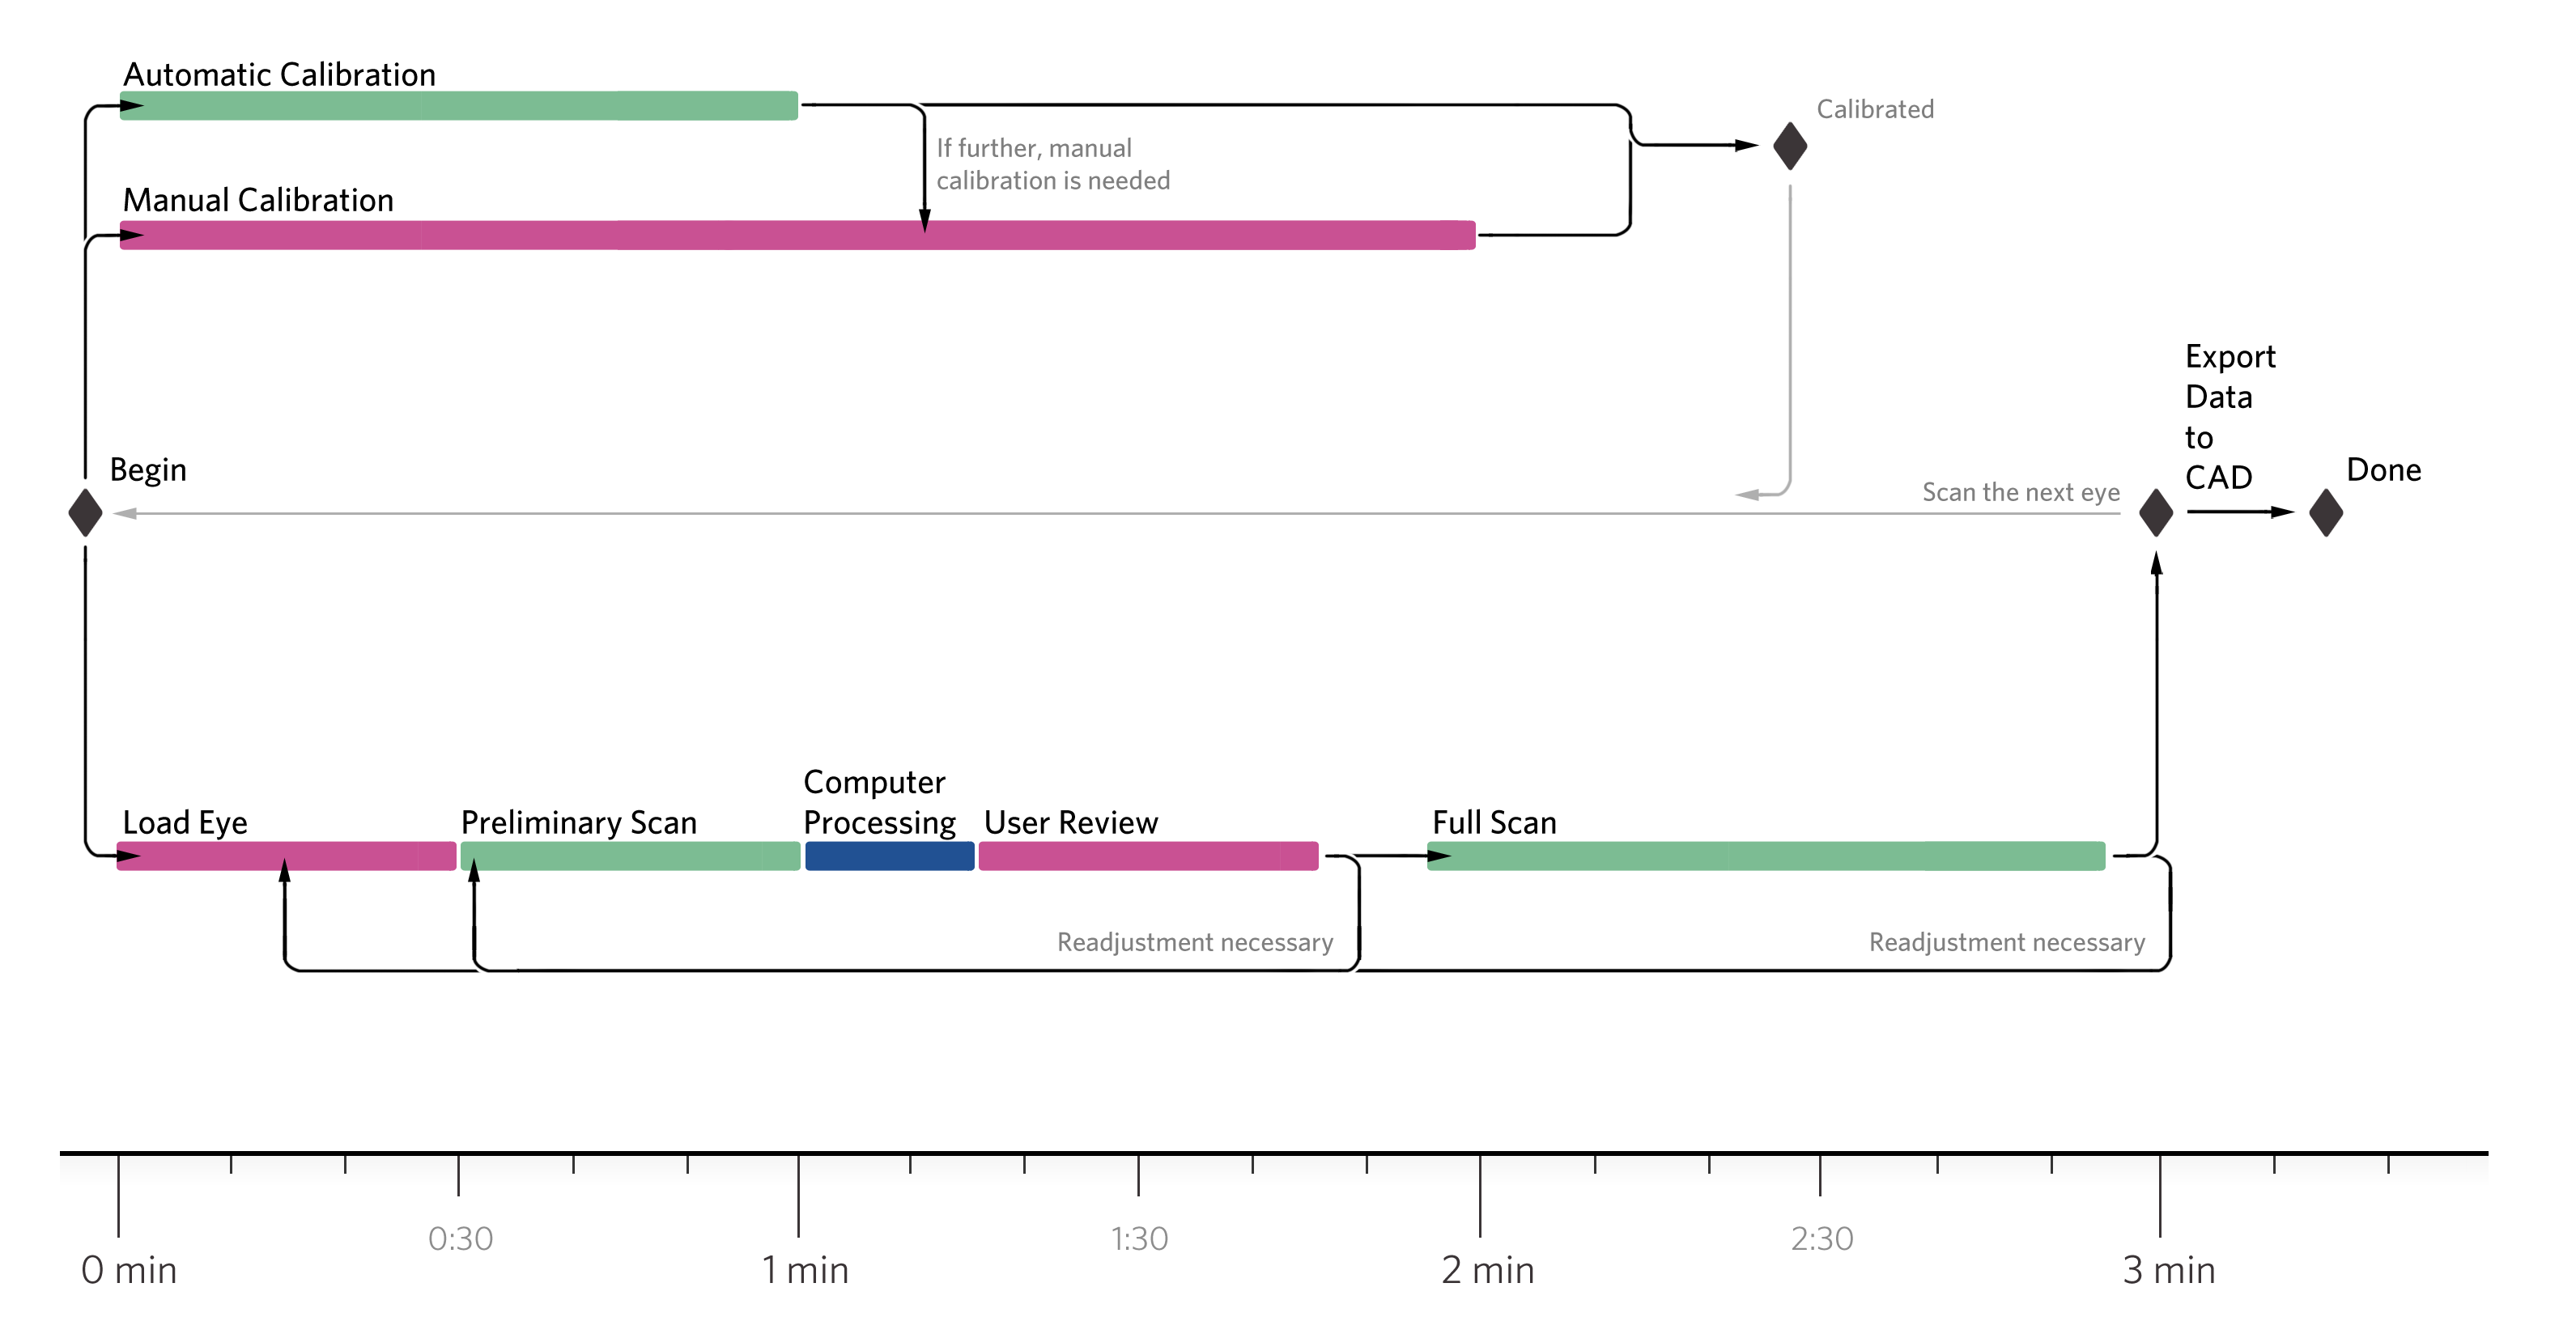
\includegraphics[width=\linewidth]{../img/usage_flow}
  \figcaption{\textbf{Possible Usage Flowchart:}  
  The device is controlled via the computer interface in order to perform a number of tasks required for repeatable, accurate measurement of an eye. Each task is located at and extended over the suggested period of time required to perform the task. Colors of the task boxes encode the required user interaction. Red tasks require direct user interaction with the physical harness, green tasks only require interaction with the computer, and blue tasks are computational tasks where the user must wait.}
  \label{fig:usage}
\end{figure}

\begin{figure}[H]
  \centering
  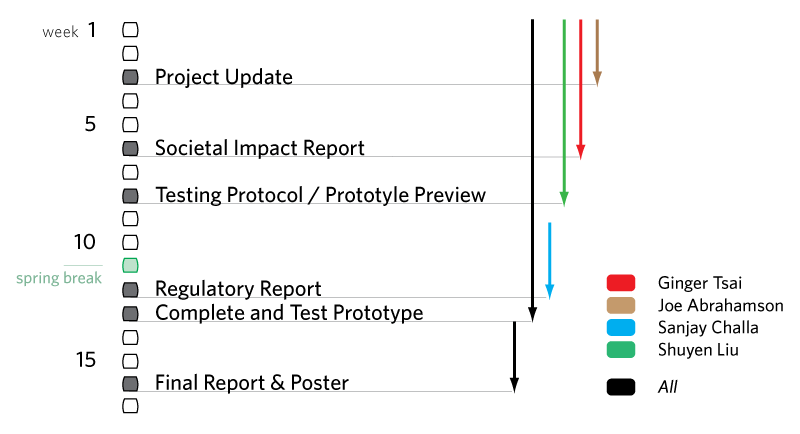
\includegraphics[width=0.75\linewidth]{../img/spring_gantt}
  \figcaption{\textbf{Gantt Chart:}
  The arrows are color coded indicating the primary author of each document. Tasks, duration of tasks, and milestones are clearly illustrated by the arrows and corresponding text at the head of each arrow.}
  \label{fig:gantt}
\end{figure}

\begin{figure}[H]
  \centering
  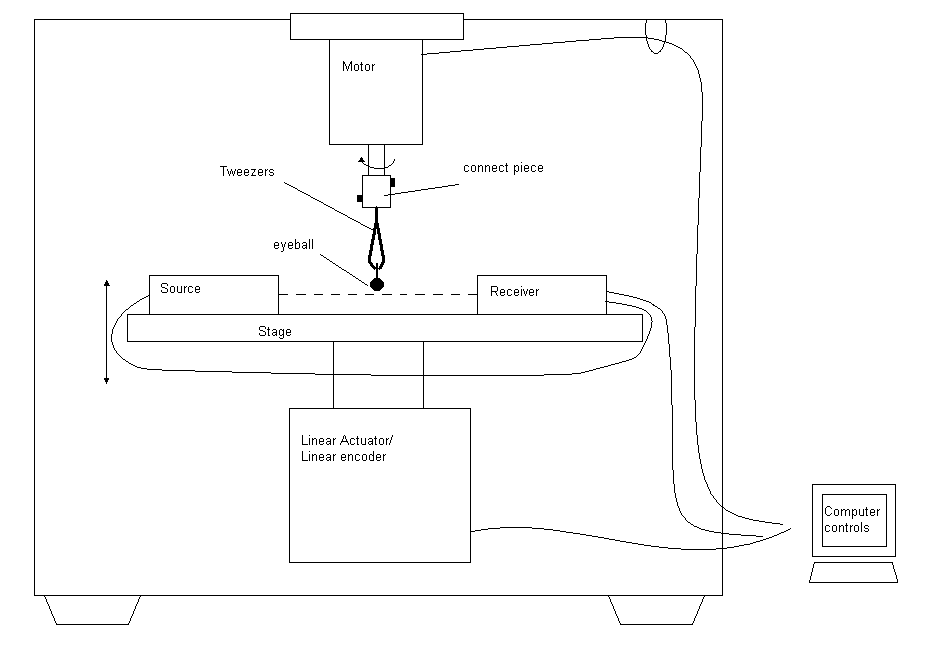
\includegraphics[width=\linewidth]{../img/schematic1}
  \figcaption{\textbf{Schematic of the Prototype:}  
  This figure illustrates the physical organization of the various components of the design within an enclosed framework. Each component is labelled. }
  \label{fig:schematic1}
\end{figure}

\newpage
\bibliographystyle{unsrt}
\bibliography{../tex/bibl}

\end{document}
